\documentclass[12pt]{article}
\usepackage{worksheet-common}
\usetikzlibrary{arrows.meta}
\definecolor{accent}{RGB}{109,91,208}
\newcommand{\ANS}[1]{\textcolor{accent}{#1}}

% Key version of electrostatics-review-notes.tex -- same structure and
% diagrams, with each blank work space replaced by a worked answer.

\begin{document}

\worksheettitle{Electrostatics Review \textcolor{accent}{(completed)} --- Flex Day, Sep 30}

%============================================================
\partsec{A}{Dipole: Torque, PE, and Motion}

\prob A uniform field $\vec E = 40$ N/C points in $+\hat x$. A dipole is made of two
$\pm3.0$ nC charges separated by $d=2.0$ mm, with its moment $\vec p$ tilted
$30^\circ$ to the right of the $y$-axis (i.e.\ $60^\circ$ from $\vec E$).

\begin{center}
\begin{tikzpicture}[x=1cm,y=1cm]
  \draw[gray,->] (-2,0) -- (2,0) node[right,scale=0.8]{$x$};
  \draw[gray,->] (0,-1.5) -- (0,2) node[above,scale=0.8]{$y$};
  \draw[cyan!60!black,->,line width=1pt] (-2.3,1.6) -- (-1.3,1.6);
  \node[cyan!60!black,scale=0.8] at (-1.8,1.9) {$\vec E$};
  \draw[thick,-{Latex[length=3mm]},accent] (0,0) -- (60:1.6) node[midway,above right,scale=0.8]{$\vec p$};
  \draw[gray!50,dashed] (0,0) -- (0,1.6);
  \draw[gray!50] (0,1.2) arc (90:60:1.2);
  \node[gray!50!black,scale=0.7] at (0.25,1.35) {$30^\circ$};
\end{tikzpicture}
\end{center}

\textbf{(a)} What is the torque on the dipole, as a vector (magnitude and direction)?

$p = qd = (3.0\times10^{-9})(2.0\times10^{-3}) = 6.0\times10^{-12}$ C$\cdot$m.
\[
\tau = pE\sin\theta = (6.0\times10^{-12})(40)\sin60^\circ = \ANS{2.1\times10^{-10}\text{ N}\cdot\text{m}}
\]
Direction: \ANS{into the page} --- $\vec\tau=\vec p\times\vec E$ points the way that
\emph{decreases} $\theta$, rotating $\vec p$ toward alignment with $\vec E$.

\textbf{(b)} What is the dipole's potential energy in this orientation?

\[
U = -pE\cos\theta = -(6.0\times10^{-12})(40)\cos60^\circ = \ANS{-1.2\times10^{-10}\text{ J}}
\]

\textbf{(c)} The dipole is released from rest and rotates until $\vec p$ aligns with
$\vec E$ (i.e.\ $\theta\to0$). Taking each charge's mass to be $m=1.2\times10^{-14}$
kg, what speed does each charge have at the instant $\theta=0$?

\textit{Hint: both charges move on a circle of the same radius about the center, so
they share the same speed --- the dipole's lost PE becomes the total KE of both
charges together.}

At $\theta=0$: $U_0=-pE=-2.4\times10^{-10}$ J. The PE lost is
$\Delta U = U(60^\circ)-U(0^\circ) = (-1.2\times10^{-10})-(-2.4\times10^{-10}) =
1.2\times10^{-10}$ J, which becomes the total KE of \emph{both} charges together:
$2\times\tfrac12mv^2 = mv^2 = \Delta U$.
\[
v=\sqrt{\frac{\Delta U}{m}}=\sqrt{\frac{1.2\times10^{-10}}{1.2\times10^{-14}}} =
\ANS{100\text{ m/s}}
\]

\clearpage
%============================================================
\partsec{B}{Even Steps in Potential, Uniform Field}

\prob A parallel-plate capacitor has plate separation $6.0$ mm and a uniform field
$E=3000$ N/C between the plates, pointing from the $+$ plate to the $-$ plate.

\textbf{(a)} Draw the field lines between the plates (evenly spaced, pointing from
$+$ to $-$).

\textbf{(b)} Draw four equally-spaced equipotential lines between the plates, and
label the potential of each one --- take $V=0$ at the negative plate.

\begin{center}
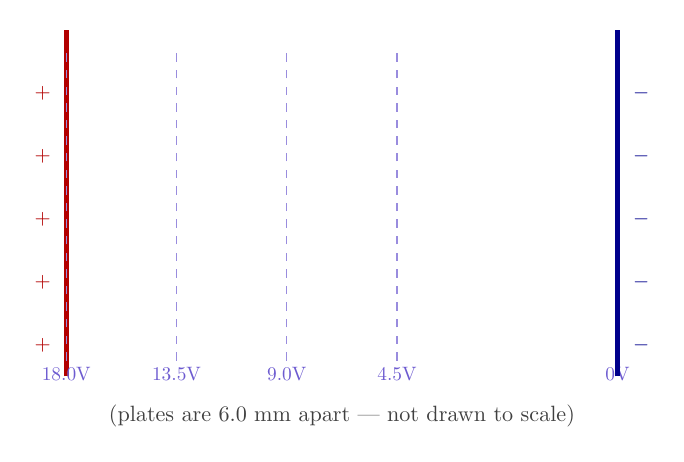
\begin{tikzpicture}[x=1cm,y=1cm]
  \draw[red!70!black,line width=1.6pt] (0,-2.2) -- (0,2.2);
  \foreach \y in {-1.8,-1.0,-0.2,0.6,1.4}{\node[red!70!black,scale=0.75] at (-0.3,\y){$+$};}
  \foreach \x/\lab in {0/{18.0},1.4/{13.5},2.8/{9.0},4.2/{4.5},7/{0}}{
    \draw[accent!70,dashed] (\x,-2.0) -- (\x,2.0);
    \node[accent,scale=0.7,below] at (\x,-2.0) {\ANS{\lab V}};
  }
  \draw[blue!55!black,line width=1.6pt] (7,-2.2) -- (7,2.2);
  \foreach \y in {-1.8,-1.0,-0.2,0.6,1.4}{\node[blue!55!black,scale=0.75] at (7.3,\y){$-$};}
  \node[gray!50!black,scale=0.8] at (3.5,-2.7) {(plates are $6.0$ mm apart --- not drawn to scale)};
\end{tikzpicture}
\end{center}
$\Delta V_{\text{total}}=Ed=(3000)(0.0060)=18.0$ V, in four \ANS{4.5 V} steps ---
the equipotentials are evenly spaced because $E$ is constant, so equal physical
steps give equal potential steps.

\textbf{(c)} A $+4.0$ nC charge moves from the positive plate to a point $1.5$ mm
away (one quarter of the way across). How much potential energy does it lose?

One quarter of the way corresponds to one $4.5$ V step ($V$ drops from $18.0$ V to
$13.5$ V):
\[
|\Delta U| = q|\Delta V| = (4.0\times10^{-9})(4.5) = \ANS{1.8\times10^{-8}\text{ J}}
\]

%============================================================
\partsec{C}{$V$ Doesn't Have to Change Evenly to Know $\Delta U$}

\prob A charge moves from point A, where $V_A=+10$ V, to point B, where $V_B=+40$ V
--- but the potential along the way is \emph{not} uniform: it rises and dips in
between (like a bumpy hill, not a smooth ramp). Sketch a plausible bumpy $V(x)$ between
A and B below, consistent with those two endpoint values.

\begin{center}
\begin{tikzpicture}[x=1cm,y=1cm]
  \draw[gray!60,->] (0,0) -- (9,0) node[right,scale=0.8]{position};
  \draw[gray!60,->] (0,-0.3) -- (0,4.5) node[above,scale=0.8]{$V$};
  \node[below,scale=0.8] at (1,-0.1) {A};
  \node[below,scale=0.8] at (8,-0.1) {B};
  \draw[gray!40,dashed] (1,0) -- (1,4.5);
  \draw[gray!40,dashed] (8,0) -- (8,4.5);
  \draw[accent,line width=1.1pt] (1,1.2) .. controls (2.3,3.4) and (2.8,0.3) .. (4,2.0)
    .. controls (5.2,3.6) and (5.6,1.0) .. (7,3.4) .. controls (7.5,4.0) .. (8,4.4);
  \node[accent,scale=0.75] at (1,0.85) {$10$ V};
  \node[accent,scale=0.75] at (8,4.7) {$40$ V};
\end{tikzpicture}
\end{center}
\ANS{Any bumpy curve is fine, as long as it starts at $10$ V and ends at $40$ V.}

\textbf{(a)} A $+2.0$ nC charge moves from A to B along this bumpy path. What is
$\Delta U$?

\[
\Delta U = q\Delta V = (2.0\times10^{-9})(40-10) = \ANS{6.0\times10^{-8}\text{ J}}
\]

\textbf{(b)} Does the bumpiness of the path matter to your answer in (a)? Why or why
not? (Think about the ball-on-a-hill analogy --- does it matter if the hill between
the start and end points is smooth or bumpy?)

\ANS{No.} $\Delta U=q\Delta V$ depends only on the potential at the two
\emph{endpoints}, never on the path between them --- exactly like a ball rolling
down a bumpy hill: only the starting and ending height set the change in
gravitational PE, no matter how many ups and downs are in between.

\clearpage
%============================================================
\partsec{D}{Superposition with Continuous Distributions}

\prob An infinite line of charge with density $\lambda=+2.0\times10^{-8}$ C/m runs
along the $y$-axis. A point charge $q=+3.0$ nC sits on the $x$-axis at $x=10$ cm.
Point $P$ sits on the $x$-axis at $x=5.0$ cm --- between the line and the point
charge.

\begin{center}
\begin{tikzpicture}[x=1cm,y=1cm]
  \draw[red!70!black,line width=1.6pt] (0,-1.6) -- (0,1.6);
  \foreach \y in {-1.2,-0.4,0.4,1.2}{\node[red!70!black,scale=0.7] at (-0.35,\y){$+$};}
  \node[red!70!black,scale=0.8] at (0,1.9) {$\lambda$};
  \draw[gray,->] (-0.7,0) -- (10.5,0) node[right,scale=0.8]{$x$};
  \node[circle,draw,fill=white,inner sep=1.5pt] at (5,0) {};
  \node[above,scale=0.8] at (5,0.2) {$P$};
  \poscharge{10}{0}{0.35}
  \node[below,scale=0.75] at (10,-0.5) {$q{=}{+}3.0$ nC};
\end{tikzpicture}
\end{center}

\textbf{(a)} Find the field at $P$ due to the line alone.

\[
E_{\text{line}}=\frac{\lambda}{2\pi\varepsilon_0 r}=\frac{2.0\times10^{-8}}
{2\pi(8.85\times10^{-12})(0.050)} = \ANS{7.2\times10^{3}\text{ N/C, in } +\hat x}
\]
(away from the line, since $\lambda>0$).

\textbf{(b)} Find the field at $P$ due to the point charge alone.

\[
E_{\text{point}}=\frac{1}{4\pi\varepsilon_0}\frac{q}{r^2}=(8.99\times10^9)
\frac{3.0\times10^{-9}}{(0.050)^2} = \ANS{1.08\times10^{4}\text{ N/C, in } -\hat x}
\]
(toward the line, since $P$ is to the left of the positive point charge, and the
field points \emph{away} from a positive charge --- away from $q$ at $P$ means
back toward the line).

\textbf{(c)} Add them as vectors (careful with directions!) to find the net field at
$P$.

\[
E_{\text{net}} = E_{\text{line}}-E_{\text{point}} = 7.2\times10^{3}-1.08\times10^{4}
= \ANS{-3.6\times10^{3}\text{ N/C (i.e.\ } 3.6\times10^3 \text{ N/C in } -\hat x\text{)}}
\]
The point charge wins, even though it's the same distance away as the line ---
these two sources just don't produce the same field strength at that distance.

\prob An infinite plane of charge with density $\eta=+1.0\times10^{-9}$ C/m$^2$ lies
in the $yz$-plane. A point charge $q=+5.0$ nC sits on the $x$-axis at $x=2.0$ cm, on
the same side as point $P$ at $x=1.0$ cm.

\textbf{(a)} Find the field at $P$ due to the plane alone, and due to the point
charge alone.

\[
E_{\text{plane}}=\frac{\eta}{2\varepsilon_0}=\frac{1.0\times10^{-9}}
{2(8.85\times10^{-12})} = \ANS{56\text{ N/C, in }+\hat x}
\]
\[
E_{\text{point}}=\frac{1}{4\pi\varepsilon_0}\frac{q}{r^2}=(8.99\times10^9)
\frac{5.0\times10^{-9}}{(0.010)^2} = \ANS{4.5\times10^{5}\text{ N/C, in }-\hat x}
\]
($r=1.0$ cm from $q$ at $x=2.0$ cm to $P$ at $x=1.0$ cm; direction is $-\hat x$
since $P$ is to the left of the positive point charge, so away-from-$q$ at $P$
points back toward the plane.)

\textbf{(b)} Add them as vectors to find the net field at $P$. Which source
dominates, and does that surprise you given how differently each one's field falls
off with distance?

\[
E_{\text{net}} = E_{\text{plane}}-E_{\text{point}} = 56 - 4.5\times10^{5}
\approx \ANS{-4.5\times10^{5}\text{ N/C (i.e.\ } 4.5\times10^5\text{ N/C in }-\hat x\text{)}}
\]
\ANS{The point charge dominates completely}, even though an infinite plane sounds
like it should be the bigger source. The plane's field never falls off with
distance, but here $P$ is extremely close to the point charge (1.0 cm) --- close
enough that $1/r^2$ wins easily over the plane's constant-but-modest field. Get far
enough away and the ranking would flip: the plane's field stays exactly the same
while the point charge's keeps shrinking.

\end{document}
